\documentclass{article}

\usepackage{amsmath}
\usepackage{fixltx2e}
\usepackage{amssymb}
\usepackage{graphicx}
\usepackage{braket}
\usepackage{esvect}
\usepackage{textgreek}

\title{Direct imaging access to habitable zone exoplanets}
\date{2017-04-21}
\author{Andrew Eberhardt\\ Mentor: Dr. B. Hicks \\ \\ GSFC Spring Internship}

\begin{document}
	\pagenumbering{gobble}
	\maketitle
	\newpage
	\pagenumbering{arabic}
	
	\section{Introduction}
		Habitable zone exoplanets are of scientific interest to NASA. Upcoming and future space telescopes will likely have the ability to directly image habitable zone exoplanets. Direct imaging offers sensitivity to a region of parameter space different than the space probed by other methods. The probability distribution for angular separation in the plane of observation (i.e. perpendicular to the line of sight) is useful to identify the probability that a planet around a given star will be observed. Additionally, in the instance where optical transmission varies with field position, the product of the probability distribution function (PDF) with the transmission function should also be considered. Here we determine the PDF as a function of angular separation in the plane of observation for the purpose of accurate Monte Carlo (MC) simulations and evaluating the probability of directly imaging habitable exoplanets with coronograph starshades. 
	
	\subsection{Orbital parameters}
	We start by assuming the star is much more massive than any of its satellites and thus deviates little from the system's barycenter. With this assumption, we can treat the orbital path of  planets as elliptical with the star stationary at one focal point. The orientation of the orbit is determined by six parameters: three Euler angles (some combination of the inclination ($i$), longitude of ascending node ($\Omega$), and argument of periapsis ($\omega$)), as well as the semi-major axis and eccentricity of the ellipse. The planet's position in three space can then be entirely determined using these parameters in addition to the true anomaly of the planet (i.e. the progress of the planet around this ellipse). For a given orbital ellipse the angular orientation of the three Euler angles is entirely arbitrary and, more importantly, isotropic. Therefore, it will suffice to solve this problem first in the plane of the orbit itself and then simply rotate it through all Euler angles to allow the orbit to occupy a random orientation. 
	
	Asserting that we are only interested in planets in the habitable zone of the star, we begin to solve the distribution. Here we define ``in the habitable zone'' as a planet being inside the habitable zone at both apastron and periastron. This restricts our possible choices of semi-major axis and eccentricity and also correlates them. While we restrict the planet to habitable zone combinations of semi-major axis and eccentricity, we want to allow the planet to occupy any arbitrary true anomaly.
	
	We define our parameters as follows:
	\begin{align*}
	&e \equiv \mbox{eccentricity of the orbit}\\
	&a \equiv \mbox{semi-major axis of the orbit}\\
	&r \equiv \mbox{star-planet separation in three-space}\\
	&\nu \equiv \mbox{true anomaly of planet}\\
	&s \equiv \mbox{star-planet apparent separation in the plane of observation}\\
	&\theta \equiv \mbox{polar angle with line of sight as reference}
	\end{align*}
	
	\subsection{Defining the habitable zone}
	
	We requires that a planet's orbit remains within the habitable zone. This does not define the bounds of the habitable zone itself. It is useful to first consider our Sun's habitable zone. Here we define our solar system's habitable zone as being between 1 and 1.68 astronomical units (au). The bounds on the habitable zones around other stars are defined as the distance at which a planet would receive the same total stellar flux as the edges of our solar system's habitable zone. The inner and outer bounds will be referred to as $a_{i}$ and $a_{o}$ respectively. The consequence of this is that both the inner and out edge of the habitable zone around other stars becomes a linear function of the root relative luminosity
	
	\begin{align*}
	&a_i = 1 \mbox{au} \sqrt{\frac{L*}{L_{sun}}} \\
	&a_o = 1.68 \mbox{au} \sqrt{\frac{L*}{L_{sun}}}
	\end{align*}
	
	This linearity is important because it means that we can parameterize our PDF's as functions of the $a_o$, giving us general results that hold for all stars regardless of type. The math in the following sections is done such that it will hold for any description of the habitable zone, not just the way we define it here. However, figures are all produced with the assumption that the habitable zone simply scales with root luminosity. 
	
	\section{Method}
	\subsection{Applying Bayes' theorem}
		What we are interested in is the PDF of \textit{s}. Using a familiar application of Bayes' theorem we can write this probability as a three dimensional integral of our parameters of interest as follows.  

	\begin{equation} \label{s}
	p(s) = \int \int \int p(s|r) p(r|a, e) p(a, e) de da dr
	\end{equation}
	
	In which the probability of each \textit{s} is given as the sum of all the possible combinations of \textit{e, a,} and \textit{r} that could result in that \textit{s} weighted by the probability of each combination occurring. The task then becomes finding each probability distribution in the integrand. It is important also to keep in mind that we want to equally weight each possible combination of \textit{e} and \textit{a}.
	
	\subsection{Evaluating the integrand}
	Here we will discuss how to find $p(s|r)$ and $p(r|a,e)$. The distribution in $e-a$ space is left for the next section on determining the bounds because it can be more easily understood from the perspective of a uniform density in \textit{e-a} space.
	
	\subsubsection{Determining three-space separation given eccentricity and semi-major axis}
	Let us turn first to the most challenging distribution; the three-space separation for a given eccentricity and semi-major axis. Applying Kepler's laws we can determine the curve of the ellipse in the plane of the orbit and its period. The orbital curve with separation given as a function of true anomaly is given as
	
	\begin{equation}
	r = \frac{a(1-e^2)}{1 + e\cos{\nu}}.
	\end{equation}
	
	Because planets traverse the curve of their orbits slower as they approach apastron, and faster as they approach periastron we cannot simply choose a random true anomaly from a uniform distribution. This is because the difference in speed means that the planet is more likely to be near apastron than periastron. We can then evaluate the PDF as function of radius (three space seperation) using the product of derivatives which we know as follows
	
	\begin{equation}\label{r_a,e}
	p(r|a,e) = \frac{dP}{dt} \left( \frac{dS}{dt} \right)^{-1}\frac{dS}{dr}.
	\end{equation}  
	
	The first derivative is the probability distribution for a given moment in the period of the orbit. Time always moves as a constant rate so this is trivially equal to the inverse of half the period. Recall that all possible radii occur twice over the entire period, and thus we only need half for the correct normalization. The second derivative represents the planets traversal of the orbital curve itself with respect to time, which is simply the speed of the planet and can be found by applying conservation of energy at a given radius. The final derivative is the arc length with respect to the radius; this can be found by using the arc length formula and the curve defining the orbit. Evaluating these derivatives we find
	
	\begin{align}
	&\frac{dP}{dt} = \frac{\sqrt{GM}}{ \pi a^{\frac{3}{2}}}, \\
	&\frac{dS}{dt} = \sqrt{GM \left( \frac{2}{r} - \frac{1}{a} \right)}, \mbox{ and} \\
	&\frac{dS}{dr} = \sqrt{1 + r^2 \frac{d\nu^2}{drr^2}} = \sqrt{\frac{r^2e^2 +2ar(1-e^2) - r^2}{r^2e^2 - (a(1-e^2) - r)^2}}.
	\end{align}

	Where \textit{G} is the gravitational constant and \textit{M} is the stellar mass (although these factors will soon cancel out). Combining these derivative as in \eqref{r_a,e} we arrive at the following expression for the conditional probability density for radial separation given an eccentricity and semi-major axis:
	
	\begin{equation} \label{r_a,e_long}
	p(r|a,e) = \frac{1}{\pi a^{3/2}}\sqrt{\frac{(2a - r)r(1 - e^2)}{(r^2e^2 - (a(1-e^2) - r)^2)\left( \frac{2}{r} - \frac{1}{a} \right)}}.
	\end{equation}
	
	It is possible, albeit somewhat cumbersome, to analytically integrate this function from $a(1-e)$ to $a(1+e)$, the full range of possible separations given a specific eccentricity and semi-major axis, which will confirm that this function is properly normalized. 
	This function can be used numerically to randomly pick three-space separations for given $e$ and $a$ (see section on MC simulation), or in a Riemann sum to evaluate equation \eqref{s}. However, when doing so one should keep in mind that equation \eqref{r_a,e_long} diverges at the maximum and minimum separations due to the diverges of $\left(\frac{dS}{dr}\right)^{-1}$ at these points. 

	
	\subsubsection{Determining angular separation given three space separation}
	In the determination of this PDF we assume that the orientation of the orbit is entirely isotropic. There is no preferred orientation and thus we would like that, for a given separation in 3-space, a uniform PDF on the surface of a sphere with radius equal to the 3-space separation. If we then break this isotropic symmetry by creating a plane of observation running through the sphere, the probability distribution associated with a given separation projected onto this plane, or apparent separation, \textit{s}, is equal to the area associated with that apparent separation divided by the total area. This is equivalent to the instantaneous area subtended by annuli on the surface of the sphere with radius \textit{s} as their thickness approaches 0. This is given as
	
	\begin{equation} \label{p(s|r)_equ}
	p(s|r) = 2 \frac{dA_{annuli}}{4 \pi r^2} = 2 \int^{2 \pi}_{0} \frac{r \sin{\theta} r d\theta}{4 \pi r^2 ds} d\phi,
	\end{equation}
	
in which $\theta$ is the polar angle and $\phi$ is the azimuthal angle in the orbital plane. Recalling that the apparent separation is given
	
	\begin{equation} \label{rsin}
	s = r \sin{\theta}
	\end{equation}
	
we find the PDF to be
	
	\begin{equation} \label{p(s|r)_full}
	p(s|r) = \frac{s}{r\sqrt{r^2 - s^2}}
	\end{equation}
	
	The integral of this function can be taken analytically, confirming that the function is properly normalized bounded between $s = [0,r]$. And while this function can be used numerically in evaluating equation (1), it diverges at $s = r$. 
	
		
	\subsection{Determining the bounds}
	\subsubsection{Determing the distribution and boundaries for eccentricity and semi-major axis}
	Recall that we desire to equally weigh every possible combination of $a$ and $e$ that fit our definition of placing a planet in the habitable zone. We know we want our perihelion to be greater than $a_{i}$ and our aphelion to be less than $a_{o}$. Using this information we can write the following inequality
	
	\begin{equation}
	a_{i} < a < a_{o}.
	\end{equation}
	
	We also want our planet to remain in the habitable zone for the duration of its orbit. Therefore, we also require 
	
	\begin{align}
	&a_{i} < a(1-e) \mbox{, and} \\
	&a(1+e) > a_{o}
	\end{align}
	
	Rearranging this we find bounds on \textit{e} as a function of \textit{a} shown in figure \ref{e vs a}.
	
	\[	
	\begin{array}{@{} r @{} c @{} l @{} }
	e_{max}(a) < 
	\begin{cases}
	1 - \frac{a_{i}}{a} & a < \frac{a_{o} + a_{i}}{2}\\
	\frac{a_{o}}{a} - 1 & a > \frac{a_{o} + a_{i}}{2}
	\end{cases}
	\end{array}
	\]
	
	\begin{figure}
		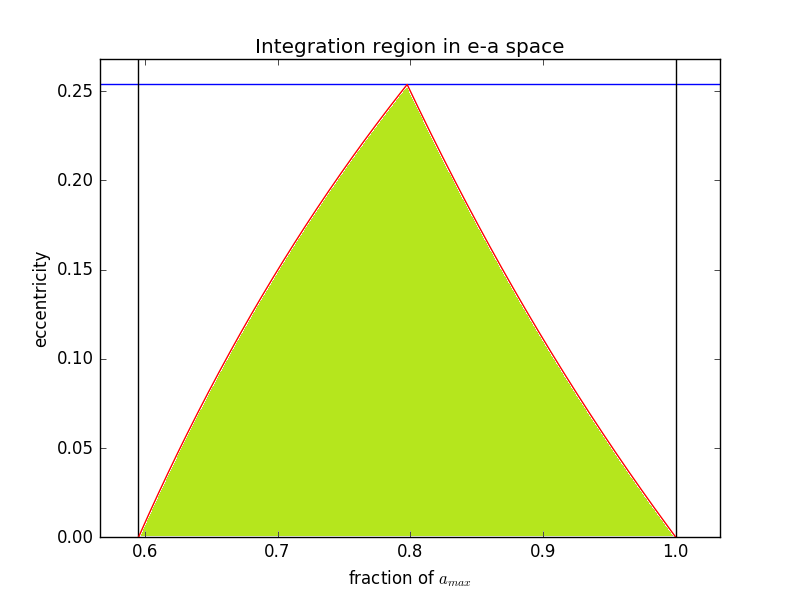
\includegraphics[width = \linewidth]{bounds_e_a.png}
		\caption{The shaded green region shows the allowed combinations of \textit{a} and \textit{e}. Vertical black lines indicate the inner and outer bounds of the habitable zone. Horizontal blue line indicates maximum allowed eccentricity (a general result for our definition of the habitable zone). }
		\label{e vs a}
	\end{figure}
	
	The shaded green region in figure \ref{e vs a} shows the allowed combinations of \textit{a} and \textit{e}. Vertical black lines indicate the inner and outer edge of the habitable zone. Horizontal blue line indicates maximum allowed eccentricity which occurs at $a_c$ (the semi major axis in the middle of the inner and outer most axes). The discontinuity occurs at the mid-point between $a_{i}$ and $a_{o}$, $a_{c}$. The maximum eccentricity is given in general as
	
	\begin{equation}
	e_{max}(a_c) = \frac{a_o - a_i}{a_o + a_i}
	\end{equation}
	
and will be constant regardless of stellar type given our definition of the habitable zone.
	
	Our probability distribution is uniform over this area. Calculating the area, we find the probability density is given 
	
	\begin{equation}
	p(e,a) = \frac{1}{a_{i}\ln{\frac{a_{i}}{a_{c}}} + a_{o}\ln{\frac{a_{o}}{a_{c}}}}
	\end{equation}
	
	At this point it is simple to set up a triple integral. The minimum and maximum range of \textit{r} can easily be written as a function of $a$ and $e$; we simply vary \textit{r} between apastron and periastron. Thus we write our distribution as follows:
	
	\begin{equation}
	p(s) = \int^{a_{o}}_{a_{i}} \int^{e_{max}(a)}_{0} \int^{a(1+e)}_{a(1-e)} \sqrt{\frac{r^2e^2 +2ar(1-e^2) - r^2}{a^{3}(r^2e^2 - (a(1-e^2) - r)^2)\left( \frac{2}{r} - \frac{1}{a} \right)(r^2 - s^2)}} C dr de da,
	\end{equation}
	
where C is a normalizing constant defined as follows
	
	\begin{equation}
	C \equiv \frac{2}{(a_{i}\ln{\frac{a_{i}}{a_{c}}} + a_{o}\ln{\frac{a_{o}}{a_{c}}})\pi^2}.
	\end{equation}
	
	From here it is possible to approximate a numerical solution for $p(s)$ with a  Riemann sum in three dimensions (\textit{a,e,r}) evaluated in a fourth dimension (\textit{s}). However, it behooves us from a computational standpoint to reduce the dimensionality of the integral. To simplify later calculations we define
	
	\begin{equation*}
	x(r,a,e,s) \equiv \sqrt{\frac{r^2e^2 +2ar(1-e^2) - r^2}{a^{3}(r^2e^2 - (a(1-e^2) - r)^2)\left( \frac{2}{r} - \frac{1}{a} \right)(r^2 - s^2)}} C
	\end{equation*}
	
	When evaluating the Riemann sum, it is important to avoid areas where the integrand diverges. Performing the Riemann sum results in the distribution shown in figure \ref{fig:p_s}.
	
	\begin{figure}
		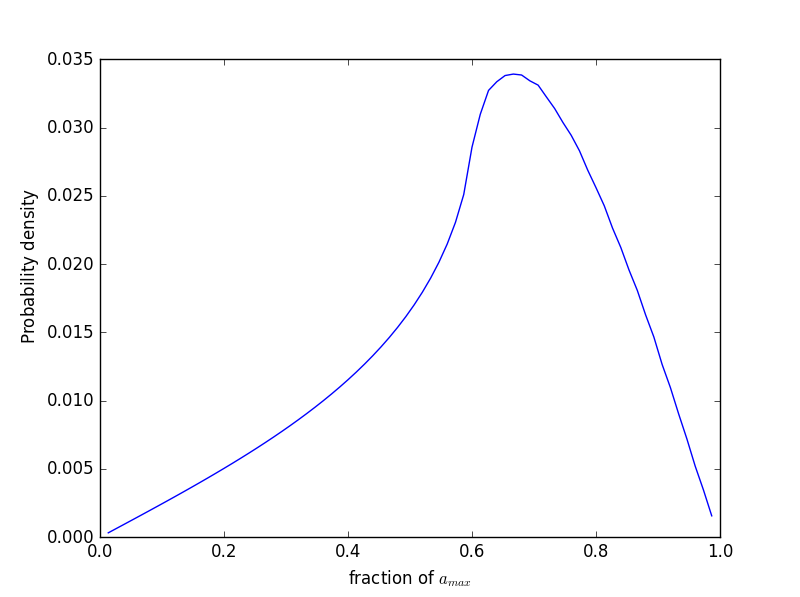
\includegraphics[width = \linewidth]{p_s_correct2.png}
		\caption{This figure shows the probability distribution function of the on-sky planet-star separation. }
		\label{fig:p_s}
	\end{figure}
	
	\subsubsection{Switching the bounds}
	The integral can be evaluated in any dimension. Integrals in \textit{r} and \textit{a} require complex numbers or special functions. It is simpler to begin by switching the bounds of our integral so that \textit{e} is the first integration.
	Right away we know the maximum and minimum values of \textit{r} and \textit{a} are $a_{o}$ and $a_{i}$ respectively. Additionally, we know for a given \textit{a} the maximum and minimum values of \textit{r} are $a(1 \pm e)$. This gives us a region of interest in the \textit{a}, \textit{r} plane shown in figure \ref{a vs r}. 
	
	\begin{figure}
		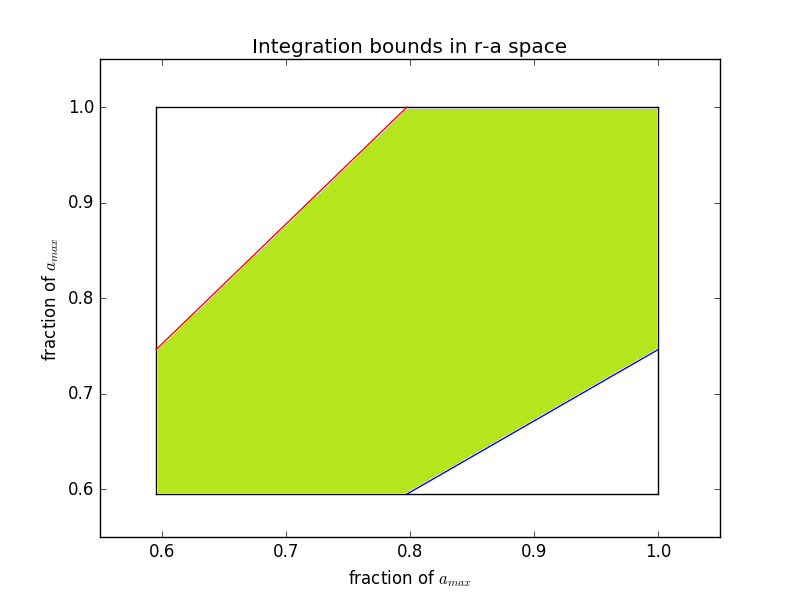
\includegraphics[width = \linewidth]{bounds_a_r.png}
		\caption{The integration region projected onto the \textit{r-a} plane. The square represents the boundaries of the habitable zone. The red and blue lines are the lines $r = a(1 + e_{max})$ and $r = a(1 -  e_{max})$ respectively. The region enclosed by all of these boundaries are shown in green and it represents the allowed combinations of \textit{a} and \textit{r}. Each line intersects the horizontal sides of the square at $a_{c}$ and intersects the vertical sides of the square at $\rho$ defined as $\rho \equiv \frac{2 a_{o} a_{i}}{a_{o} + a_{i}}$.}
		\label{a vs r}
	\end{figure}

	Note that \textit{s} must be less than \textit{r}, which intuitively makes sense as there is no orientation that would result in the on-sky separation exceeding the actual three space separation, and is also evident from the form of $p(s|r)$. Reinterpreting these bounds in the new order gives us the sum of the following four integrals:
	
	\begin{equation}
	p(s) = X_1 + X_2 + X_3 + X_4
	\end{equation}
	
	Defined as 
	
	\[	
	\begin{array}{@{} r @{} c @{} l @{} }
	X_1(r, a, e, s) \equiv 
	\begin{cases}
	\int^\rho_{a_{i}}\int^\frac{r}{1 - e_{max}}_{a_{i}} \int^{e_{max}}_{|r/a - 1|} x de da dr  & s < a_{i}\\
	0  &  else
	\end{cases}
	\end{array}
	\]

	\[	
	\begin{array}{@{} r @{} c @{} l @{} }
	X_2(r, a, e, s) \equiv 
	\begin{cases}
	\int^\rho_{s}\int^\frac{r}{1 - e_{max}}_{a_{i}} \int^{e_{max}}_{|r/a - 1|} x de da dr  & a_{i} < s < \rho\\
	0  &  else
	\end{cases}
	\end{array}
	\]
	
	\[	
	\begin{array}{@{} r @{} c @{} l @{} }
	X_3(r, a, e, s) \equiv 
	\begin{cases}
	\int^{a_{o}}_\rho \int^{a_{o}}_\frac{r}{1 + e_{max}} \int^{e_{max}}_{|r/a - 1|} x de da dr  & s < \rho \\
	0  &  else
	\end{cases}
	\end{array}
	\]
	
	\[	
	\begin{array}{@{} r @{} c @{} l @{} }
	X_4(r, a, e, s) \equiv 
	\begin{cases}
	\int^{a_{o}}_s \int^{a_{o}}_\frac{r}{1 + e_{max}} \int^{e_{max}}_{|r/a - 1|} x de da dr  & \rho < s < a_{o} \\
	0  &  else
	\end{cases}
	\end{array}
	\]
	
	\subsection{Evaluating the integral in eccentricity space}
	Note that the bounds in eccentricity space are the same in each of the integrals above (11). Thus, it will suffice to solve 
	
	\begin{equation*}
	\int^{e_{max}}_{|r/a - 1|} x(r,a,e,s) de
	\end{equation*}
	
	Evaluating it in the region of interest we find it is equal to 
	
	\begin{equation}
	C \sqrt{\frac{r(2a - r)}{a^5(2/r - 1/a)(r^2 - s^2)}}\ln{\left( \frac{|a - r|}{\sqrt{a^2(e_{max}^2 - 1) + 2ra - r^2} +ae_{max}} \right)}
	\end{equation}
	
	Which can then be evaluated with a Riemann sum much faster as we no longer need to sum in e-space. When evaluating numerically one should notice the integrand now diverges along $r = a$.
	
	\section{Evaluating via Monte Carlo}
	Evaluating the on-sky separation distribution via integration has a number of drawbacks. For example, the integrand diverges along many of the boundaries, it is time consuming to do via Riemann sum, and complicated to do with an analytical solution because of the introduction of complex valued terms. Evaluating the distribution via Monte Carlo (MC) offers an alternative method that avoids many of these problems. 
	
	\subsection{Monte Carlo method}
	We begin the MC treatment of the problem by randomly, and uniformly picking an \textit{a} and \textit{e} from our allowed region, shown in figure \ref{e vs a}. Given a semi-major axis and eccentricity we can now pick from our $p(r|a,e)$ distribution (equation \eqref{r_a,e_long}). Keep in mind that this distribution diverges at the maximum and minimum values of \textit{r}, however this problem can be easily solved by simply setting a high ceiling on the probability density value. At this point, one can either choose randomly from the distribution $p(s|r)$ using the same caution at the diverging points or simply randomly and uniformly pick a value for $\theta$ between 0 and $\pi/2$ and use equation \eqref{rsin} to convert this angle to an on-sky separation. Figure \ref{fig:MC} shows the PDF obtained by repeating this process a billion times, giving us .01\% accuracy. 
	
	\begin{figure}
		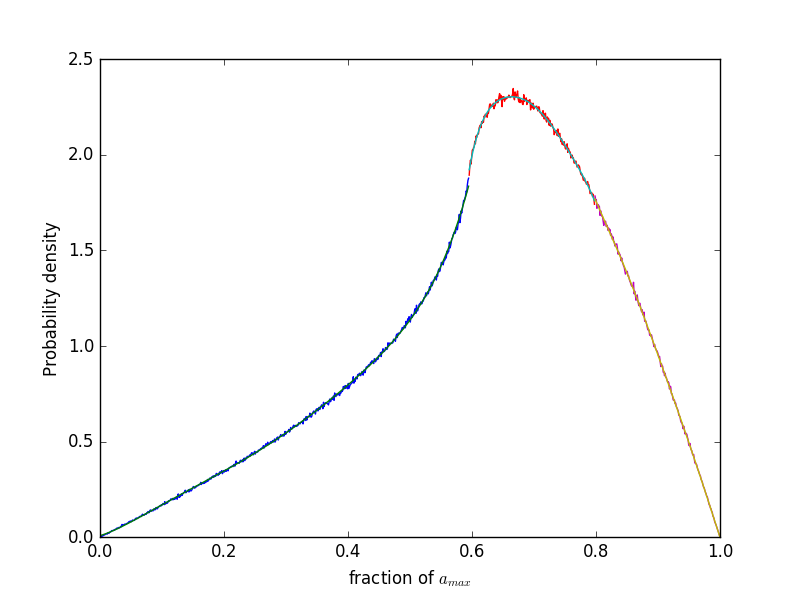
\includegraphics[width = \linewidth]{MC_corrected.png}
		\caption{MC estimations of probability distribution function. The bottom axis is on-sky separation in au. Vertical axis is probability per .0168 au. Results are separated by color into three regions. Blue is for $s<a_{min}$, red $a_{min} < s < a_{c}$, and purple $a_{c} < s$. }
		\label{fig:MC}
	\end{figure}
	
	\subsection{Monte Carlo method uncertainties}
	We can think of our probability distribution function evaluated via MC simulation as a series of bins in which a number of events occurs, where the number of events that occurs in a given bin is a random variable. Thus, with each bin there is some “true” proportion of events that fall into that bin out of the total events simulated. This proportion is itself the value of the probability distribution function at that bin multiplied by the bin size. The proportion we measure with the MC simulation must then follow a binomial distribution for each bin. If the bin resolution is fine enough that the “true” proportion of events to fall in a given bin is small compared to the entire number of events (which should be the case for 1000 bins as in our simulation) then we can estimate the binomial distribution as a Poisson distribution for each bin with Poisson parameter equal to the “true” expectation value of the bin. We therefore define some terms as follows
	
	\begin{align*}
	&\pi \equiv \mbox{true proportion of events that should occur in a given bin}\\
	&N_{tot} \equiv \mbox{total number of trials}\\
	&N_{tot}\pi = \braket{N} \equiv \mbox{true number of events that should occur in a given bin}\\
	&N_i \equiv \mbox{total number of events that actually occurred in a given bin}.
	\end{align*}
	
	Using the fact that $N_i$ follows a Poisson distribution with $\braket{N}$ expectation value, we can then say the standard deviation on our estimation of $\braket{N}$ goes as $\sqrt{\braket{N}}$. Dividing by $N_{tot}$ to convert to a proportion, we find our estimation of $\pi$ must goes as $\pi /\sqrt{N_{tot}}$.We can see that our estimation of the true value of the proportion in each bin then must improve as $\sqrt{N_{tot}}$. The accuracy of this method is then limited by the number of trails we can run. For a billion trials our confidence interval is reduced by four and a half orders of magnitude, meaning we are left with an estimate of our true distribution accurate to .01\%. 
	
	The variance for the measured proportion, \textit{p}, as a function of the true proportion, $\pi$ is just the variance for a binomial distribution, which is
	\begin{equation}
	var(p) = \pi(1. - \pi),
	\end{equation}

and is maximal at $\pi = .5$ (where the stand deviation is also 0.5, or just the entire span of possible values), obviously, the true proportion of events that occur in any one of 1000 bins is going to be much smaller than 0.5 but we can put an upper bound on the variance using this method. Thus we expect, for a billion trials, the standard deviation for each bin to be bounded as follows 
	\begin{equation}
	\mbox{standard deviation for $\pi$} < \frac{.5}{\sqrt{N_{tot}}} = 1.6 x 10^{-5}
	\end{equation}

	
	\section{Evaluating a transmission probability distribution function}
	\subsection{Multiple shear transmission functions}
	In our field of view of our simulated nulling interferometer the interference pattern created by splitting and recombining light changes the transmission PDF as a function of simulated separation. We can shear this light before recombination and thus introduce phase difference in the recombined beams. Here we show the transmission pattern in the field of view that results from multiple shears. Transmission is proportional to the square of the electric field at a given point. We define some variable as follows
	
	\begin{align*}
	&\vec{s}_j \equiv \mbox{the vector representing a given shear in units of fraction of the aperture radius}\\
	&E_j \equiv \mbox{the electric field resulting from a given shear}\\
	&\vec{r} \equiv \langle x, y \rangle \\
	&D \equiv \mbox{the aperture diameter} \\
	&\lambda \equiv \mbox{ the observation wavelength}\\ 
	\end{align*}
	
	Making the simplifying assumption that all light rays will be equal magnitude, we can always simply normalize our fields. The initial un-sheared electric field is treated as a vector in the complex plane of unit length whose phase with respect to some fixed axis is a function of position on the field of view and time. We typically choose to orient phasors with respect to the positive real axis but this is simply a choice of gauge. Any observables will be unchanged under the addition of a phase factor $e^{i \delta}$ (where $\delta$ is real), which trivially preserves the length of our vector and simply adds an additional rotation. We then have initial electric field as follows
	
	\begin{equation}
	E_0 \propto e^{\left( \Phi(r,t) + \delta\right) i}
	\end{equation}
	
where $\Phi(r,t)$ is some real function defined at every $r$ and $t$. We set $\delta = \Phi(r,t)$. Now the initial electric field is defined as being fixed on the positive real axis. You can think of this as transforming into the frame of the rotating arrow in the complex plane. This is an appropriate transformation because, in this derivation, we are not interested in the way our initial electric field varies over time and space only how our sheared fields vary with respect to it.
	Recombining an electric field with a shear simply takes the old field and adds it to itself with an additional phase factor of $e^{\frac{2 \pi \vec{r} \cdot\vec{s}_j i D}{\lambda} + i \pi}$, where the first part of the argument represent the phase introduced by the shear and the second part represents the phase introduced to create destructive interference. The field from the jth shear can then be represented as 
	
	\begin{equation}
	E_j \propto e^{\frac{2 \pi \vec{r} \cdot\vec{s}_j i D}{\lambda} + i \pi} \sum_{k = 0}^{j-1} E_k,
	\end{equation}
	
and the total electric field is a sum of all the fields resulting from shears and the original field. 
	
	\begin{equation*}
	E_t \propto \sum^{N_{s}}_{j = 0} E_j.
	\end{equation*}
	
$N_s$ is the total number of shears. Because each new term in the sum includes all the previous terms, but with an additional phase factor, it can be shown that this result factors to
	
	\begin{equation*}
	E_t \propto \prod^{N_s}_{j = 1} (1 - e^{\frac{2 \pi \vec{r} \cdot\vec{s}_j i D}{\lambda}}).
	\end{equation*}
	
Finally, taking the complex square, we find, for an arbitrary amount of shears, the transmission pattern is given as follows
	
	\begin{equation}
	T(x,y) = \prod^{N_s}_{j = 1} \sin^2{\frac{\pi D \vec{r} \cdot\vec{s}_j }{\lambda}}.
	\end{equation}
	
	
	\subsection{Hexagonal shear transmission}
	Now that we have a probability distribution function for on-sky separation, we can randomly pick from our distribution in \textit{s} and uniformly pick from a uniform distribution for $\phi$ to randomly generate a position in the sky. This position can be converted to an angular separation by dividing by the special resolution of our telescope. We can then calculate the transmission (T) at that point in the sky. The transmission pattern we are interested in is for a dual-nulling interferometer with two shears. 	We choose two shears as follows
	
	\begin{align}
	&\vec{s}_1 = \frac{1}{9} \langle 0,1 \rangle \\
	&\vec{s}_2 = \frac{1}{18} \langle \sqrt{3}, 1 \rangle
	\end{align}
	
this fraction is intended to represent a shear that covers a single row of mirror segments in the planned aperture of LUVOIR. Resulting in a transmission pattern (figure 5) governed by 
	
	\begin{equation}
	T(x,y) = \sin^2{\frac{\pi D y}{9 \lambda}} \sin^2{\frac{\pi D (\sqrt{3}x + y)}{18 \lambda}}.
	\end{equation}
	
	\begin{figure}
	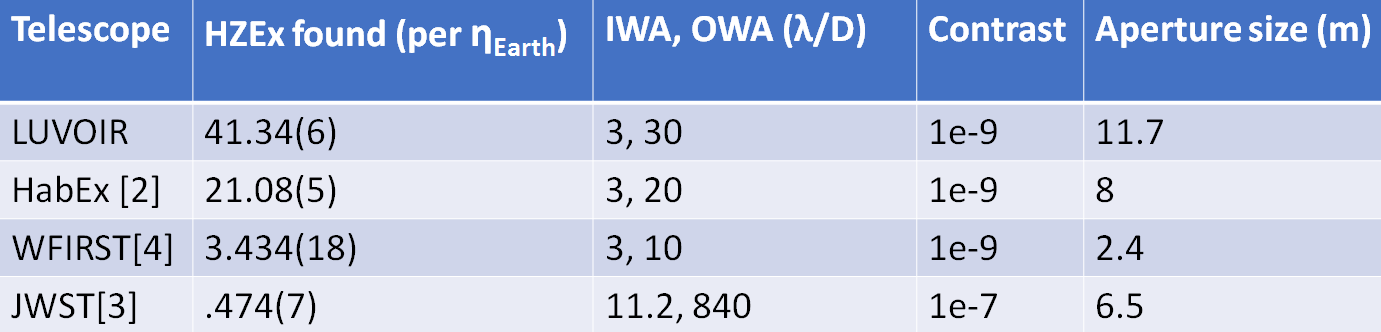
\includegraphics[width = \linewidth]{telescope_table.png}
	\caption{A summary of assumptions made about the performance of future telescopes.}
	\label{fig:telescope}
	\end{figure}
	
	\begin{figure} 
		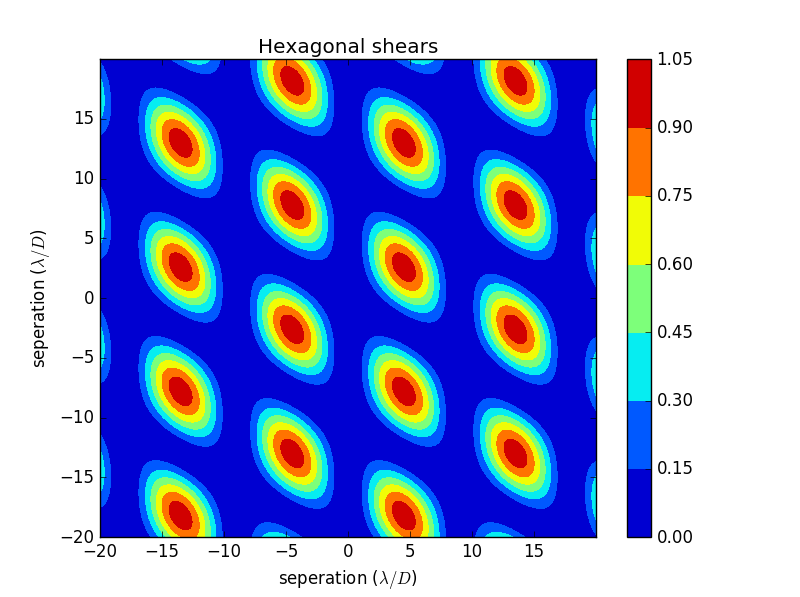
\includegraphics[width = \linewidth]{T_xy.png}
		\caption{The on-sky transmission function of a nuller following a hexagonal shear. Warm colors represent higher transmission, cool colors represent less.}
		\label{fig:T_xy}
	\end{figure}
	
The inner four peaks of the transmission function are at $\left( \pm \frac{9 \lambda}{2 \sqrt{3} D}, \pm \frac{9 \lambda}{2 D} \right)$ and $\left(\pm \frac{27 \lambda}{2 \sqrt{3} D}, \mp\frac{9 \lambda}{2 D} \right)$ and lie on the ellipse $\frac {x^2}{54} + \frac{\sqrt{3} xy}{81} + \frac{5 y^2}{162} = 1$.
	
	We run a MC simulation to find the transmission distribution function. The results for $\tau$ Ceti at .76 $\mu m$ (a prominent O2 line) and a million trials (resulting in .1\% error bars) with 11.7 meter aperture diameter is shown in figure \ref{fig:p_T} see our table on telescope assumptions. 0 transmission is assigned if the on-sky separation falls inside the inner working angle or outside the outer working angle. The outer working angle is based on the expected performance of LUVOIR, and the inner working angle is defined as the angular distance to the nearest point of half-maximum transmission.There values are
	
	\begin{align*}
	&IWA =  \frac{18}{\sqrt{3}\pi}\arcsin{\left(\frac{1}{2}\right)^{\frac{1}{4}}}\frac{\lambda}{D} \approx 3.30 \frac{\lambda}{D}\\
	&OWA = 30 \frac{\lambda}{D}
	\end{align*}
	
	\begin{figure}
		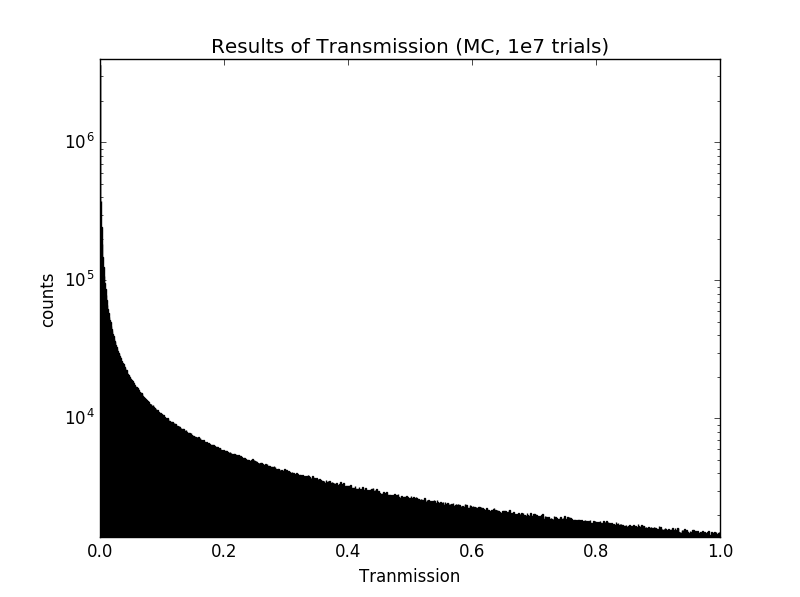
\includegraphics[width =\linewidth]{p_T.png}
		\caption{The results of a MC simulation with a million trials for Tau Ceti at .5$\mu m$ with a 6.5 meter aperture diameter (see telescope table).}
		\label{fig:p_T}
	\end{figure}
	
the average transmission is $.13915 \pm .00046$ and the probability of 0 transmission is $.01470 \pm .00012$. IWA is defined by the 50\% constructive peak, OWA defined by deformable optics. Figure \ref{fig:T v wl} and \ref{fig:z v wl} shows the average transmission and probability of 0 transmission, for the same system, as functions of wavelength.
	
	\begin{figure}
		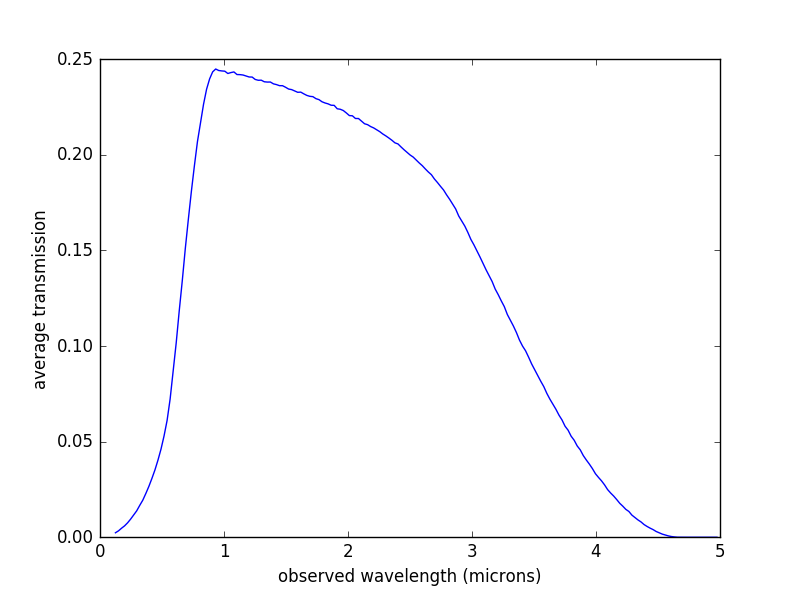
\includegraphics[width = \linewidth]{T_wl.png}
		\caption{The average transmission plotted as a function of observation wavelength for Tau Ceti with a 6.5 meter aperture diameter.}
		\label{fig:T v wl}
	\end{figure}
	
	\begin{figure}
		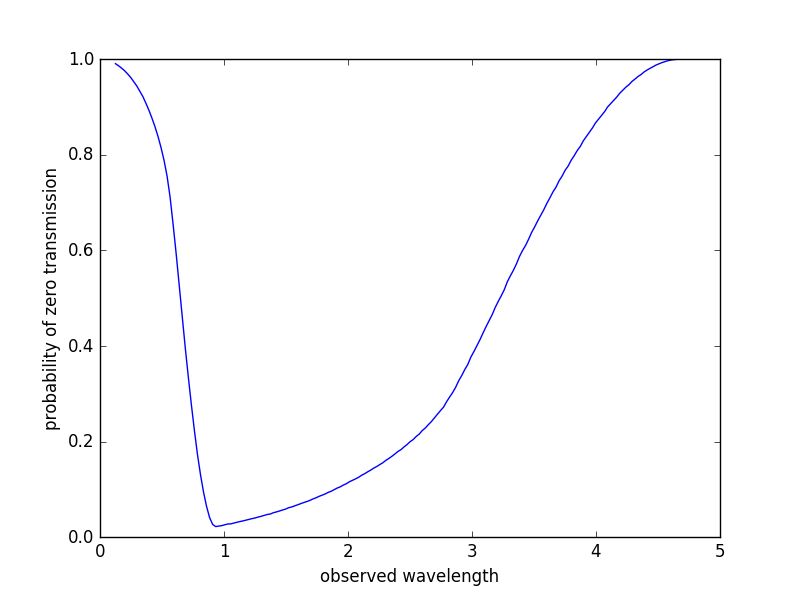
\includegraphics[width = \linewidth]{z_pi_wl.png}
		\caption{Probability of 0 transmission was a function of observation wavelength for Tau Ceti with 6.5 meter aperture diameter.}
		\label{fig:z v wl}
	\end{figure}
	
	\subsection{Transmission of two parrallel shears}
	Now we choose two parallel shears in the $\hat{y}$ or $\hat{x}$ direction. Proceeding as we did before, we find the transmission pattern is given by 
	
	\begin{align}
	&\vec{s}_1 = \frac{1}{9} \langle 0,1 \rangle \\
	&\vec{s}_2 = \frac{1}{9} \langle 0,1 \rangle \\
	&T(x,y) = \sin^4{\frac{\pi D y}{9 \lambda}}
	\end{align}

with $IWA = \frac{9}{\pi}\arcsin{\left(\frac{1}{2}\right)^{\frac{1}{4}}} \frac{\lambda}{D} \approx 2.86 \frac{\lambda}{D}$. The resulting transmission pattern is shown in figure \ref{fig:T_xy2}. Average transmission is $0.25168 \pm 0.00021$ and chance of total obscuration is $0.079833 \pm 0.000086$.
	
	\begin{figure}
		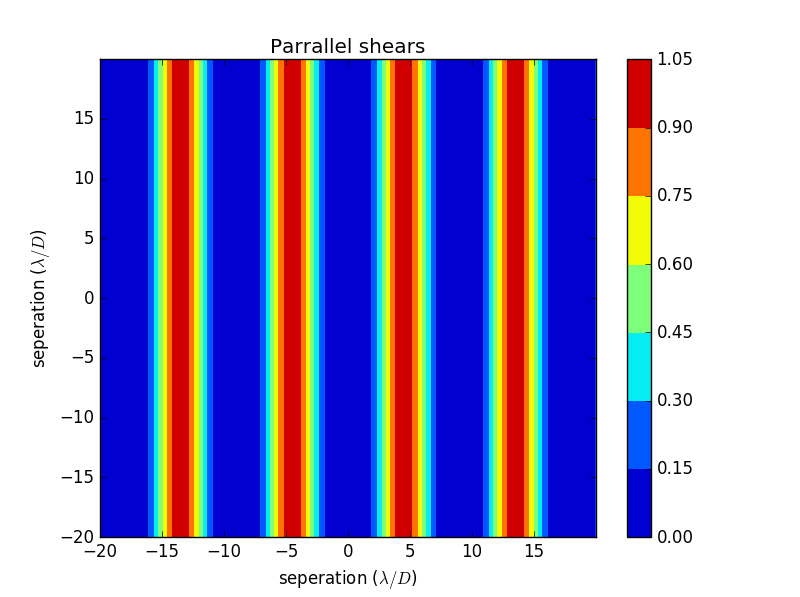
\includegraphics[width = \linewidth]{T_xy2.png}
		\caption{ Shows the transmission pattern for parallel shears. Warm colors represent higher transmission, cool colors represent less. Axis are in units of $\lambda/D$.}
		\label{fig:T_xy2}
	\end{figure}
	
	\section{Evaluating the sensitivity of specific telescopes}
	
	\subsection{Telescope assumptions}
	
	\begin{figure}
	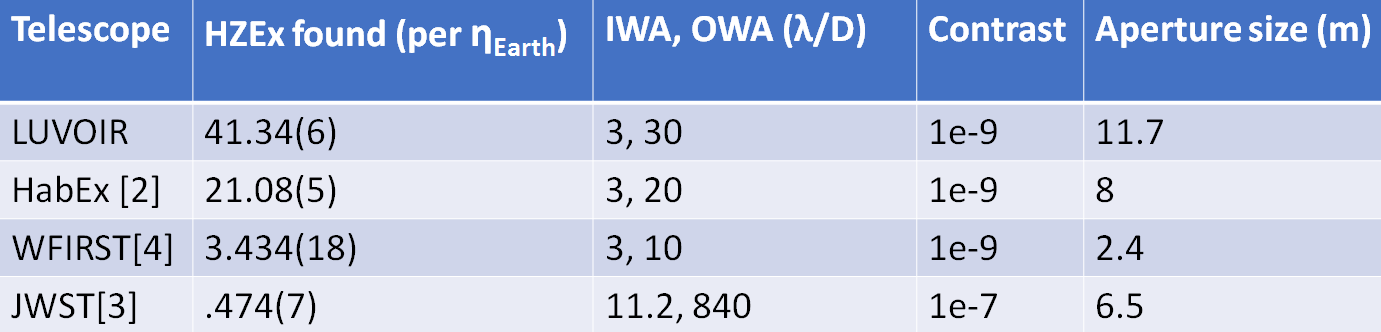
\includegraphics[width = \linewidth]{telescope_table.png}
	\caption{A summary of assumptions made about the performance of future telescopes.}
	\label{fig:telescope}
	\end{figure}
	
	When discussing the results of simulations in the following sections it is important to note the assumptions made about the telescopes hardware and observational capabilities. Table summarizing these assumptions \ref{fig:telescope}.
	
	\subsection{Defining an observation parameter}
	
	Because the probability distribution function for the on-sky separation can be written as a function of  fractions of $a_{o}$ without loss of generality, the only thing that is going to determine the specific observational sensitivity of a given instrument is how the angular on-sky separation compares with the instrument’'s angular resolution. Therefore we define the dimensionless parameter 
	
	\begin{equation}
	x \equiv \frac{\lambda d}{D a_o}
	\end{equation}
	
in which $d$ is the distance to the system. For a given instrument the PDF for on-sky separation will scale with this parameter as the IWA and OWA stay constant (or vice versa). This concept is illustrated in figure \ref{fig:A_x}.
	
	\begin{figure}
		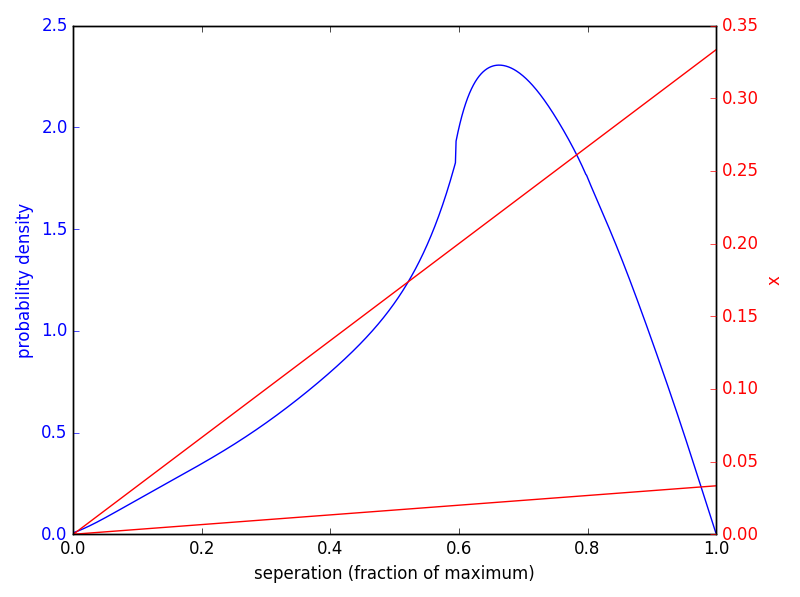
\includegraphics[width = \linewidth]{angles_pdf_LUVOIR.png}
		\caption{This plot shows how IWA and OWA compare with our on-sky PDF as a function of $x$. The two red lines are superimposed on the probability distribution function for on-sky separation. For a given value of $x$ corresponding to some star, the separation on each line corresponding to that $x$ value indicates the position of the $IWA$ and $OWA$ relative to the PDF for on-sky separation. Each angle is exactly equal to the maximum separation at an $x$ value of one over its radius in units of $\lambda / D$.}
		\label{fig:A_x}
	\end{figure}
	
	$x$ is a parameter unique to a given telescope observing a specific star. It will also be useful later to work with a parameter that is unique to a specific star irrespective of the observing instrument, thus we define another dimensionless parameter 
	
	\begin{equation}
	x_{intrinsic} \equiv \frac{x D}{\lambda} = \frac{d}{a_o},
	\end{equation}
	
	which is essentially the inverse of the angle the maximum habitable separation makes on the sky. 
	
	Using these parameters, it is easy to determine the probability that a star with a given x value will be within our field of view. We use figure \ref{fig:A_x} to determine the bounds for our field of view and integrate our PDF from the IWA to the OWA as
	
	\begin{equation}
	p(\mbox{in} | x) = \int^{OWA(x)}_{IWA(x)} p(s) ds
	\end{equation}
	
	This function is plotted in figure \ref{fig:p_in_x} along with a histogram of stars within 30 pc as a function of their $x$ values. 
	
	\begin{figure}
		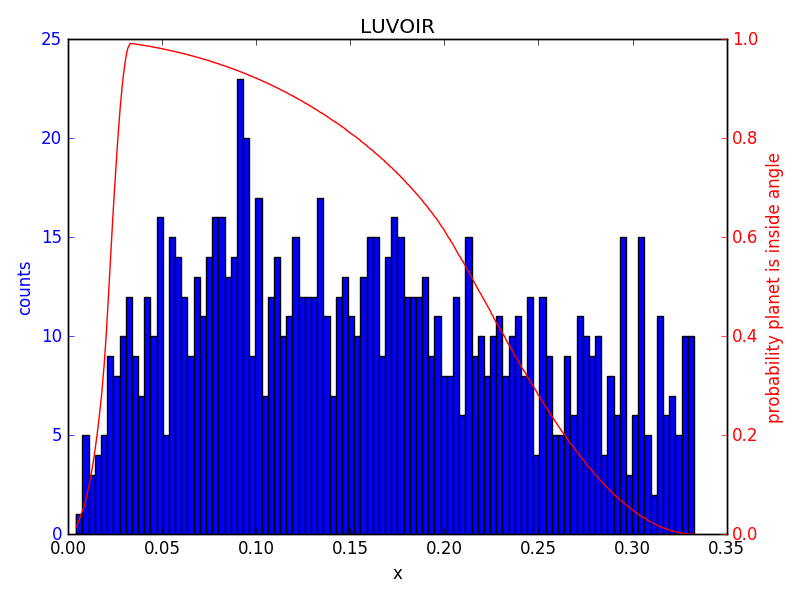
\includegraphics[width = \linewidth]{LUVOIR_planet_expect.png}
		\caption{The probability a habitable zone planet (the red curve) inside the field of view as a function of observation parameter for a 11.7 m telescope observing at .76 $\mu$m. The blue histogram shows star counts within 30 pc as a function of observation parameter.}
		\label{fig:P_x_LUVOIR}
	\end{figure}
	
	\subsection{Capability of future telescopes}
	
	Using the technique discussed in the previous section we evaluate the probability of a habitable planet being inside the field of view for all stars with in 30 pc that have a non-zero probability of being observed by LUVOIR, JWST, and WFIRST at .76 microns. We use IWA 3, 11.2, and 3 for LUVOIR, JWST and WFIRST respectively with OWA 30, 840 and 10. The probability of a habitable zone planet being inside the field of view is shown in figure \ref{fig:telescopes} as a function of $x_{intrinsic}$ for each telescope. 
	
	\begin{figure}
		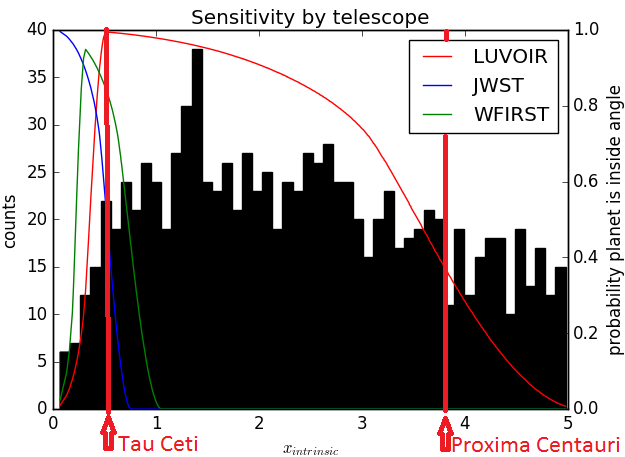
\includegraphics[width = \linewidth]{all_planet_expect_labeled.png}
		\caption{The probability of being inside the field of view for each telescope as a function of $x_{intrinsice}$ over 1e6.The histogram is for all stars in 30 pc with a non-zero probability of being observed by one of the telescopes. The $x_{intrinsic}$ values for \texttau \ Ceti and Proxima Centauri are labeled for reference.}
		\label{fig:telescopes}
	\end{figure}
	
	We can then say that if we were to observe each star the number of habitable zone planets we would expect to observe would go as follows
	
	\begin{equation}
	\braket{N_H} = \int_{\mbox{all}} f(x) p(\mbox{in}|x) p(\mbox{obs}|\mbox{in}) \eta_H(x) dx
	\end{equation}
	
	where 
	
	\begin{align*}
	&N_H \equiv \mbox{number of observed habitable zone planets} \\
	&f(x) \equiv \mbox{function describing the number of observed stars with given x value} \\
	&p(\mbox{obs}|\mbox{in}) \equiv \mbox{the probability of observing a planet given that it is in the field of view} \\
	&\eta_H(x) \equiv \mbox{the true proportion of stars with given x value that have habitable zone planets}
	\end{align*}
	
	$N_H$ follows a Poisson distribution. A goal of exoplanet observations is to determine $\eta_H$. Unfortunately for a given instrument, $\eta_H(x)$ is exactly convolved with $p(\mbox{obs}|\mbox{in})$ which is non-trivial and the focus of other works. However if we assume that both are approximately uniform over $x$ then we can remove them from the integral. What we are left with is simply the dot product of the $p(\mbox{in}|x)$ with the histograms for stars as a function of $x$. We can then define the observational opportunity of a given instrument ($\xi$)) as this integral. 
	
	\begin{equation}
	\xi \equiv \int_{\mbox{all}} f(x) p(\mbox{in}|x) dx
	\end{equation}
	
	This integral represents the total number of planets we would expect to observe if we surveyed every possible star and perfectly found every star within our field of view and every star had a habitable zone planet. We can then rewrite our equation as 

	\begin{equation}
	\braket{p(\mbox{obs}|\mbox{in}) \eta_H} = \frac{\braket{N_H}}{\xi}
	\end{equation}
	
 $p(\mbox{obs}|\mbox{in})$ cannot be removed because we do not know its value. However,  if we could, this equation could be used to put constraints on the true value of $\eta_H(x)$. And even now we can show the relative ability of each telescope to constrain their product. The product itself represents the fraction of planets we found out of the total we would expect to find if we surveyed every possible star and perfectly found every star within our field of view and every star had a habitable zone planet. $p(\mbox{obs}|\mbox{in}) \eta_H$ does not exactly follow the distribution for proportions we discussed earlier (because it is not bounded by 1), but the uncertainty in the true value of $p(\mbox{obs}|\mbox{in}) \eta_H$ will still fall as $1/\sqrt{\xi}$ because our expectation value for the number of events is linear with $\xi$ and Poisson distributed. Thus it is worth determining $\xi$ for each telescope. They are 532.1, 35.5, and 58.0 for LUVOIR, JWST and WFIRST respectively. Of course our ability to constrain the value of $\braket{p(\mbox{obs}|\mbox{in}) \eta_H}$ depends on what the value actually is but LUVOIR will constrain the true value by about half an order of magnitude better than the other telescopes.
	A prediction interval (PI) will tell us the region in which measurements of an estimator are likely to lie. In this case the estimator is  $\widehat{p(\mbox{obs}|\mbox{in}) \eta_H}$ which estimates the true value of our paramter $p(\mbox{obs}|\mbox{in}) \eta_H$. We run a MC simulation Poisson-selecting a number of observed habitable zone exoplanets and calculate a PIl of our estimator as a function of the true value of our parameter. The PI is centered at the true value of the parameter, which indicates that our estimator has statistical consistency, and its width is a function of the true value of the parameter and $\xi$. The width of the PI is a measure of our ability to estimate the true value of our parameter, i.e. a narrow PI indicates a better ability to estimate the parameter. Figure \ref{fig:PI_} shows the PI as a function of the true value of the parameter. These intervals are constructed such that 95\% of measurements of our estimator will lie within the interval. Figure \ref{fig:width} shows the width of the interval as a function of the true value of the parameter.
	
	\begin{figure}
		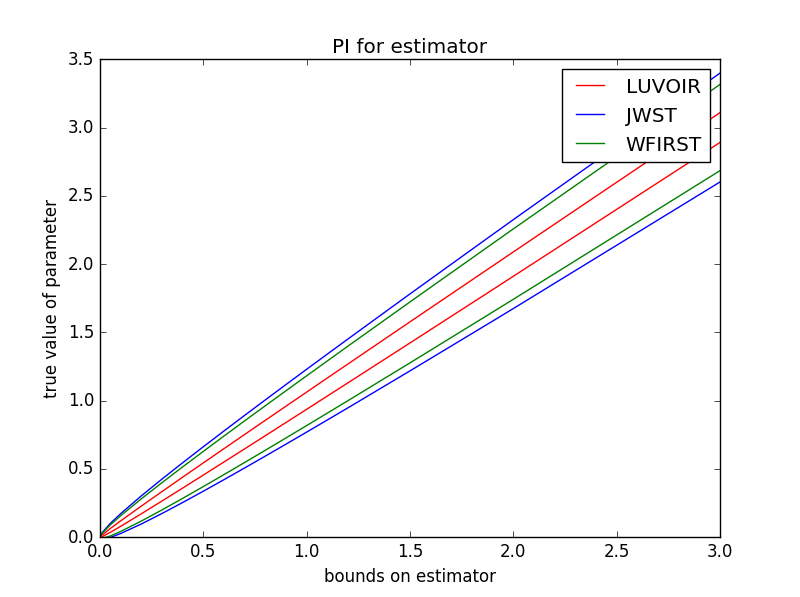
\includegraphics[width = \linewidth]{PI_eta.png}
		\caption{The upper and lower bounds for mission as a function of the true value of the parameter. For a given true value of $p(\mbox{obs}|\mbox{in}) \eta_H$, 95\% of measurements of $\widehat{p(\mbox{obs}|\mbox{in}) \eta_H}$ will land inside the two lines.}
		\label{fig:PI_}
	\end{figure}
	
	\begin{figure}
		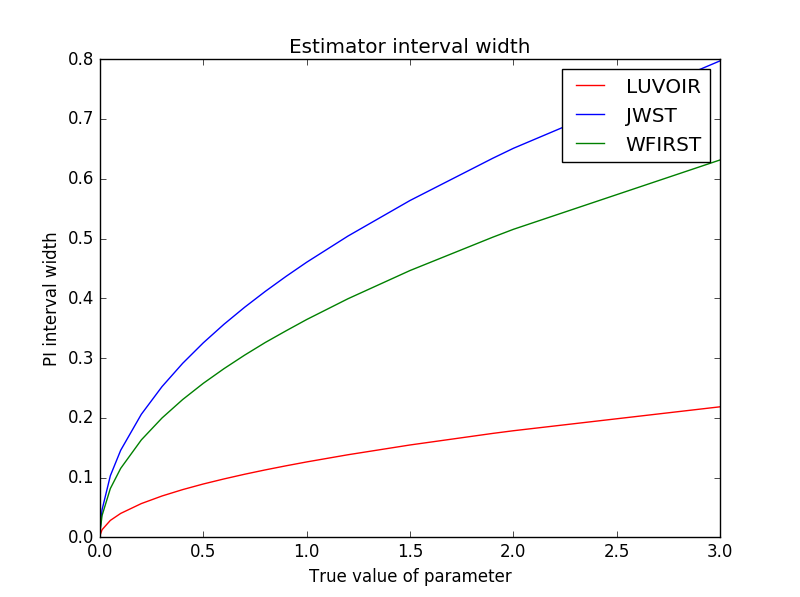
\includegraphics[width = \linewidth]{PI_width_eta.png}
		\caption{The width of the PI as a function of the true value of our parameter. The width grows as the root of the true value, as expected of variables following Poisson statistics.}
		\label{fig:width}
	\end{figure}
	
	\section{Prioritization and sensitivity simulations}
	\subsection{Simulation overview}
	
	We run simulations of observation campaigns looking at habitable zone exoplanets around nearby stars. The simulations all follow the same basic framework with respect to observing a given planet around a star, which is outlined in this section. All planets are assumed to have Earth-radii and albedo. An orbit is generated around a target star with a random semi major axis and eccentricity such that the orbit fits our definition of a habitable zone orbit. 
	We then ``collect photons'' from the star and planet as follows
	
	\begin{align}
	&\braket{N_{planet}} = \Phi A \frac{L_{*}}{4 \pi r^2} \frac{\pi R_{earth}^2}{4 \pi d^2} \frac{\pi D^2}{4} \frac{\lambda}{h c} f_L dt \\
	&\braket{N_{*}} = C \frac{L_{*}}{4 \pi d^2} \frac{\pi D^2}{4} \frac{\lambda}{h c} f_L dt
	\end{align}
	
where $\braket{N}$ defines the expectation value for the number of photons being collected (the actual number measured follows Poisson statistics. The other variables are defined as follows
	
	\begin{align*}
	&\Phi \equiv \mbox{the phase factor, i.e. fraction of the light being reflected by the planet towards observer} \\
	&A \equiv \mbox{the albedo of the planet} \\ 
	&R_{earth} \equiv \mbox{Earth's radius} \\
	&h \equiv \mbox{Planck's constant} \\ 
	&c \equiv \mbox{the speed of light} \\
	&f_L \equiv \mbox{the fraction of light in the bandpass} \approx \frac{2 \pi h \delta \lambda c^2}{\sigma \lambda^5 T^4 \left( \exp{\left( \frac{h c}{\lambda k T} \right)} - 1  \right)} \\
	&\delta \lambda \equiv \mbox{width of bandpass} \\
	&T \equiv \mbox{Stellar temperature} \\
	&k \equiv \mbox{Boltzmann constant}\\
	&\sigma \equiv \mbox{Stephan-Boltzmann constant} \\
	&dt \equiv \mbox{integration time}
	\end{align*}
	
the number of photons received from the planet is added to a running total of ``signal photons'' ($S$) collected. The number of planet photons and stellar photons are added to a running total of ``background photons'' ($B$). These running totals are then converted to a z score corresponding to the number of standard deviations the signal is above the background as follows 
	
	\begin{equation}
		z = \frac{S - B}{\sqrt{B}}
	\end{equation}
	
	Here, a z score over 5 is considered a detection (this has a false alarm rate of about 3 in 1e5). The orbit is then progressed by $dt$. This is done approximately using a Riemann sum of Keplers second law; i.e. iterating the orbital angle until an area approximately equal to $dt/\mbox{P}$ is swept out by the orbital curve. 
	This process is repeated until the mission lifetime has expired or the alloted time for observing the given star has expired.
	
	\subsection{Simulations investigating expected integration times}
	
	\begin{figure}
		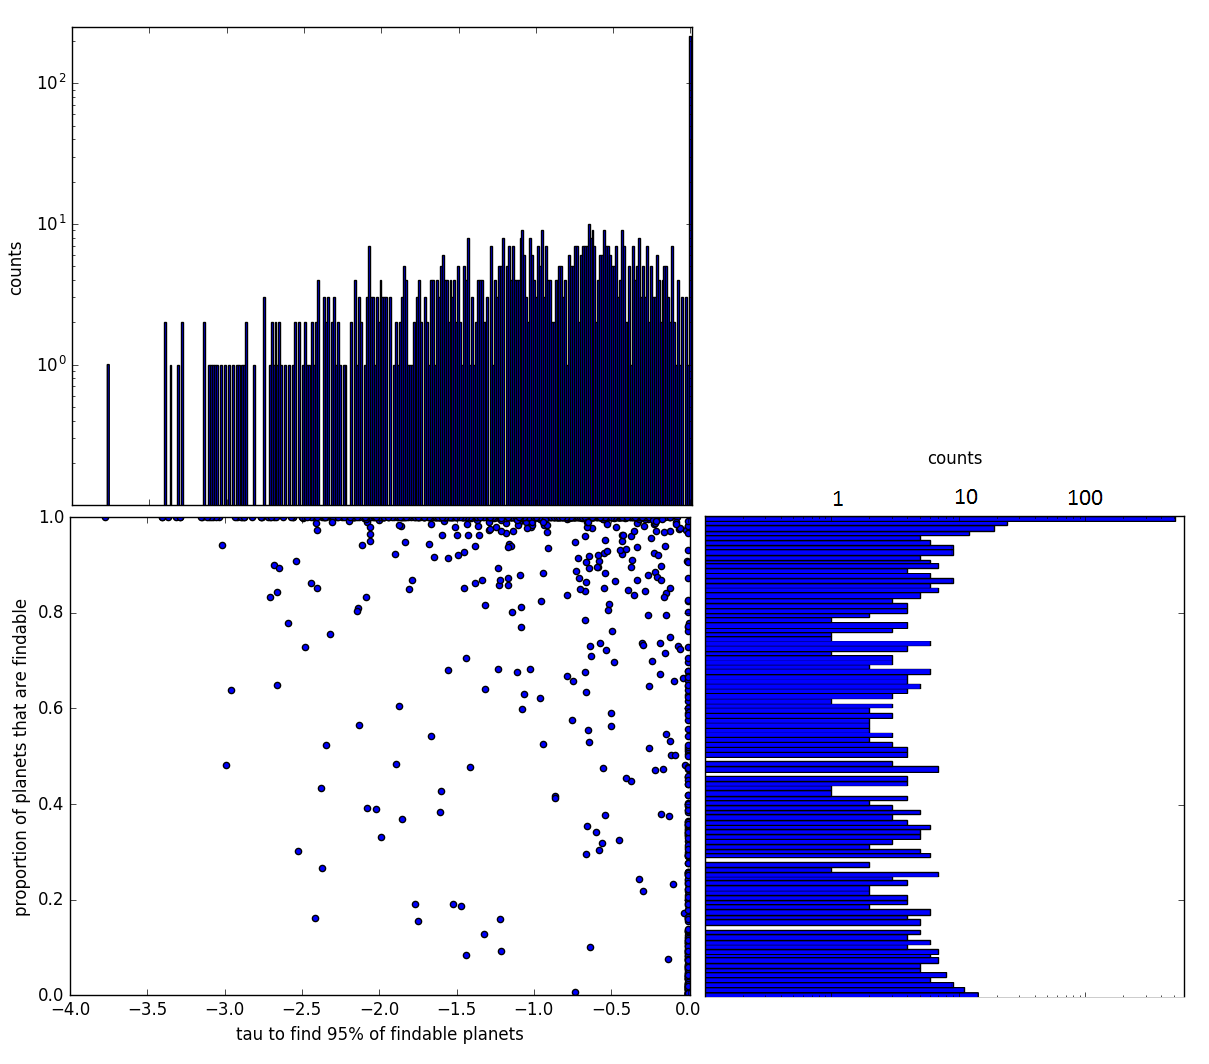
\includegraphics[width = \linewidth]{findable_v_tau_ex_LUVOIR_composite.png}
		\caption{Lower left, a scatter plot of stars according to their $\tau_{ex}$ times and proportion of detectable planets for LUVOIR.}
		\label{fig:LUVOIR_tau_ex}
	\end{figure}
	
	\begin{figure}
		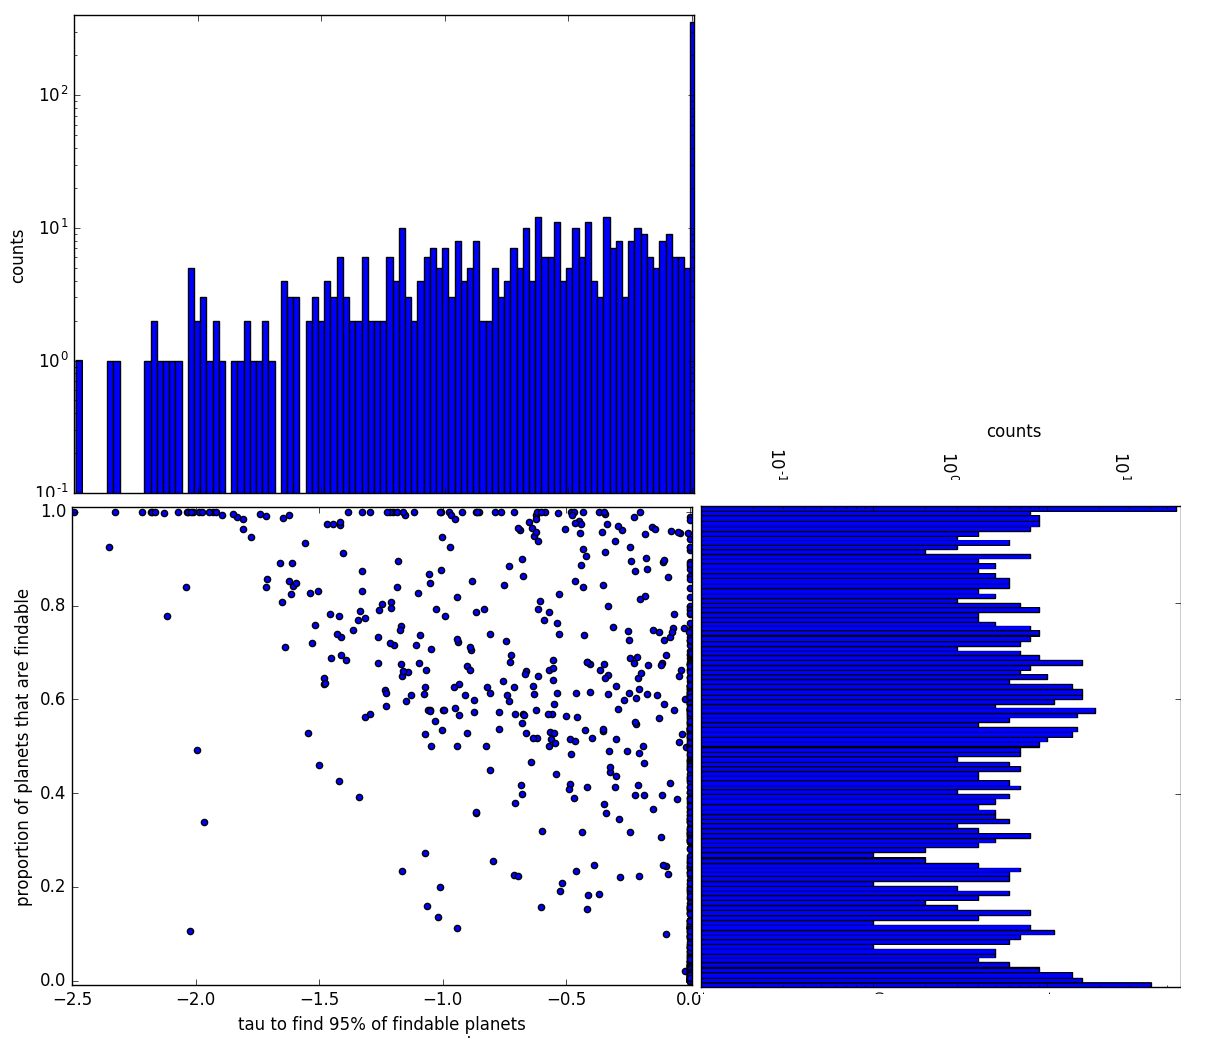
\includegraphics[width = \linewidth]{findable_v_tau_ex_HABEX_log.png}
		\caption{Lower left, a scatter plot of stars according to their $\tau_{ex}$ times and proportion of detectable planets for HabEx.}
		\label{fig:HABEX_tau_ex}
	\end{figure}
	
	\begin{figure}
		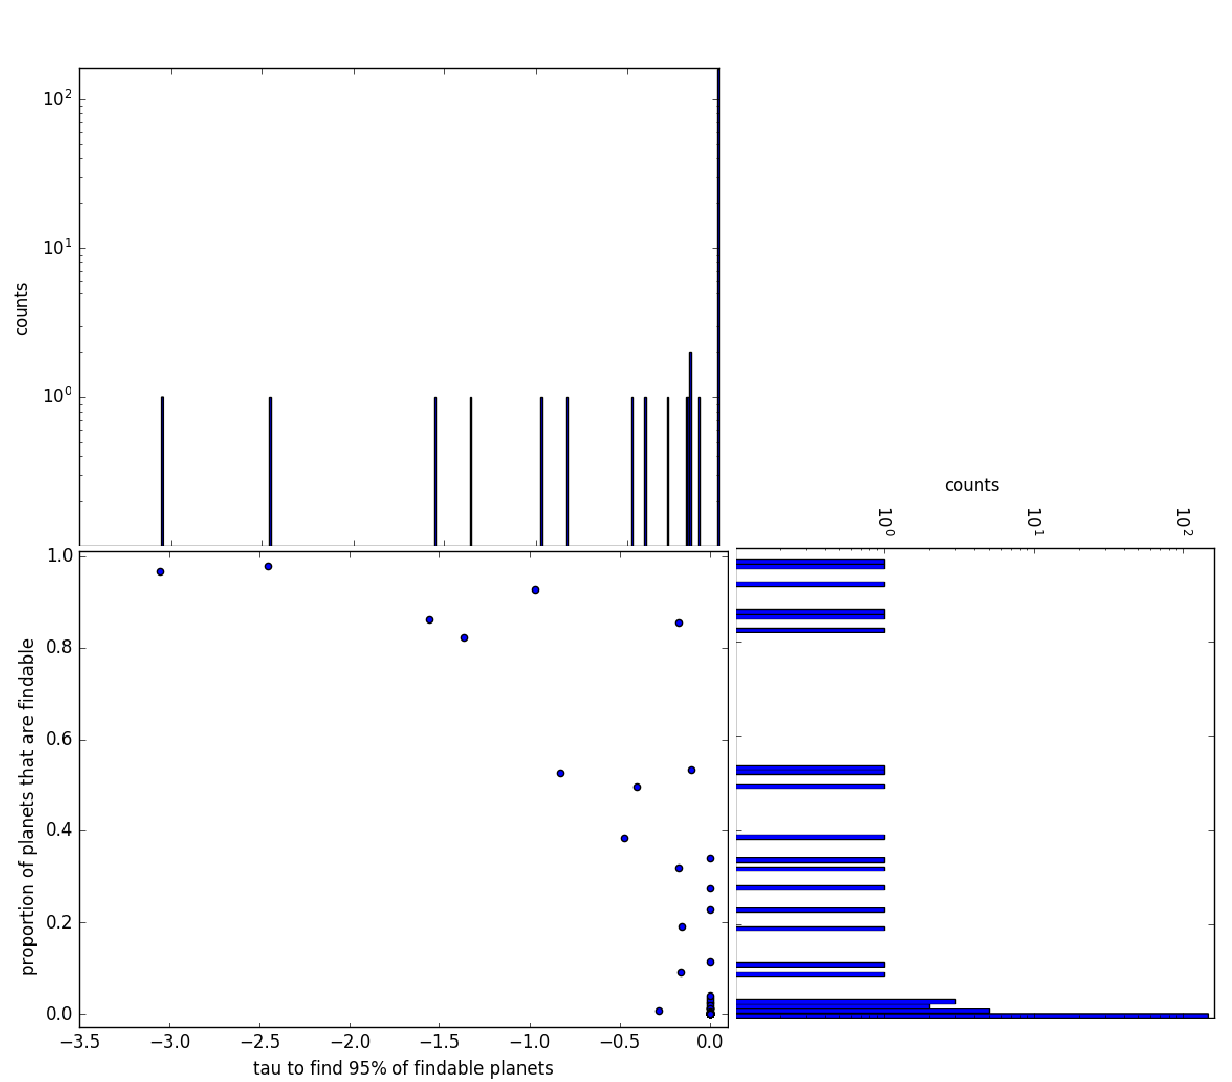
\includegraphics[width = \linewidth]{findable_v_tau_ex_WFIRST_composite.png}
		\caption{Lower left, a scatter plot of stars according to their $\tau_{ex}$ times and proportion of detectable planets for WFIRST.}
		\label{fig:WFIRST_tau_ex}
	\end{figure}
	
	\begin{figure}
		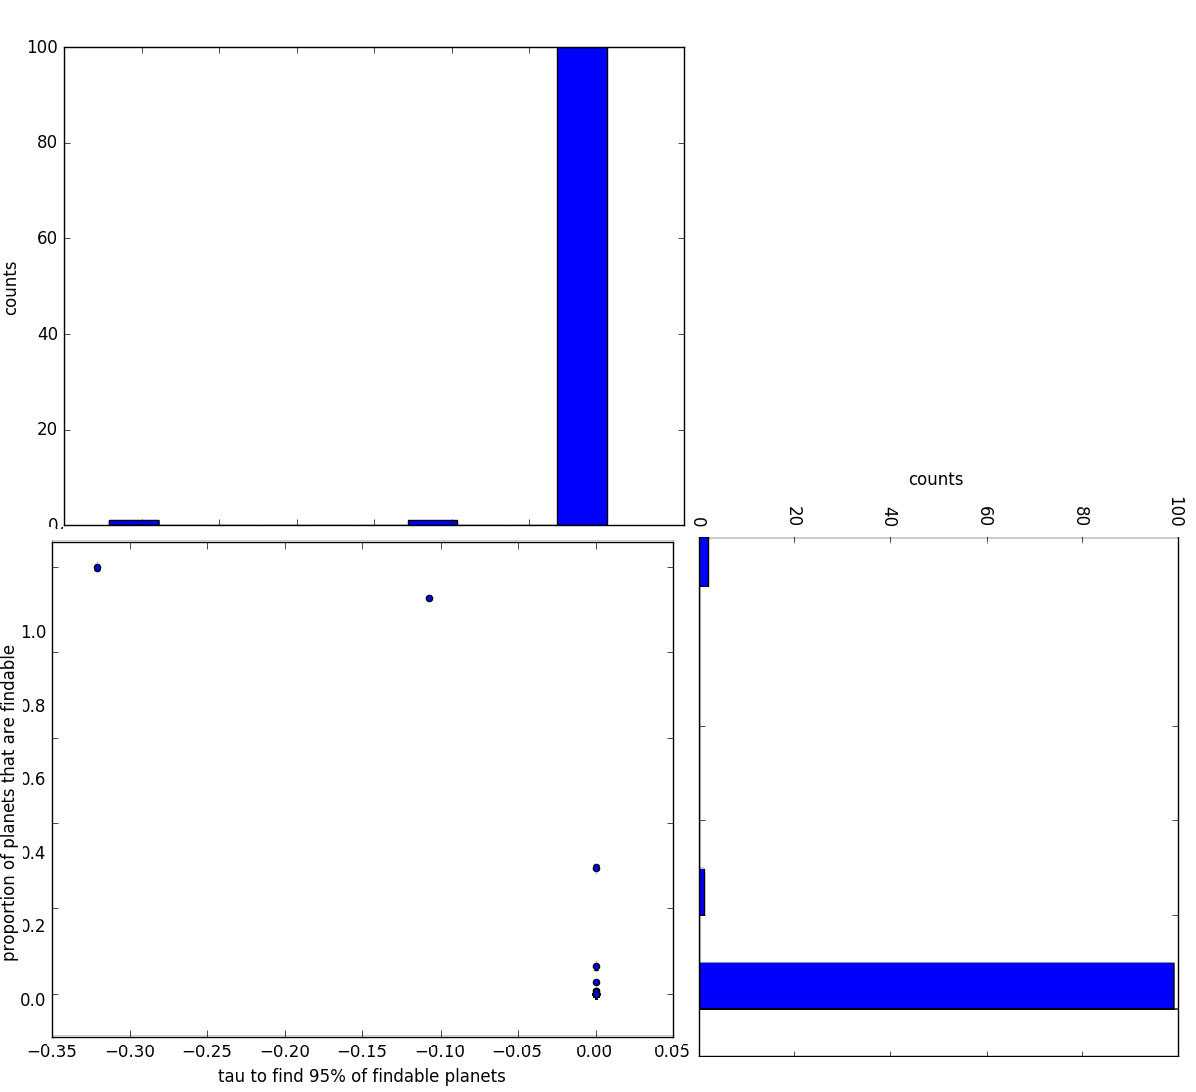
\includegraphics[width = \linewidth]{findable_v_tau_ex_JWST_composite.png}
		\caption{Lower left, a scatter plot of stars according to their $\tau_{ex}$ times and proportion of detectable planets for JWST.}
		\label{fig:JWST_tau_ex}
	\end{figure}
	
	We simulate random planets around all stars within 30 pc with a non-zero chance of having an observable habitable zone exoplanet and calculated the integration time required to detect each planet (capped at a year). For each star we determined the 95th percentile integration time for detecting planets that had integration times less than $\tau_{ex}$. We can then say that if a given star is observed for its $\tau_{exclude}$ you can be 95\% confident that you will either detect a habitable zone exoplanet (with Earth radii and albedo) around that star or 95\% confident that there exist no habitable zone exoplanets around that star that can be detected in less than our cap time ($t_{max}$).
	The proportion of planets that are detectable in less than $t_{max}$ is also recorded for each star, $P_{detect}$. The results of this exercise are given in figures \ref{fig:LUVOIR_tau_ex}, \ref{fig:HABEX_tau_ex}, \ref{fig:WFIRST_tau_ex}, and \ref{fig:JWST_tau_ex}. Stars would be prioritized for observation based on a parameter $y$ defined as follows (lower $y$ values correspond to higher priority). All simulations use assumptions explained in table \ref{fig:telescope}.
	
	\begin{equation}
		y \equiv \frac{\tau_{ex}}{P_{detect}}
	\end{equation}
	
	\subsection{Observation campaign simulations}
	
	\begin{figure}
		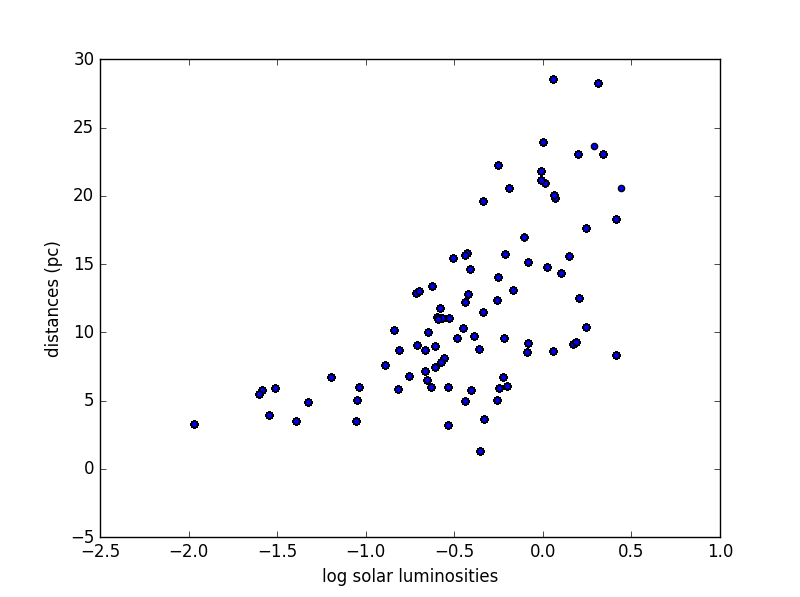
\includegraphics[width = \linewidth]{LUVOIR_d_L_scatter.png}
		\caption{A scatter plot of the stars around which habitable zone exoplanets were detected in these simulations with LUVOIR.}
		\label{fig:LUVOIR_dL}
	\end{figure}
	
	\begin{figure}
		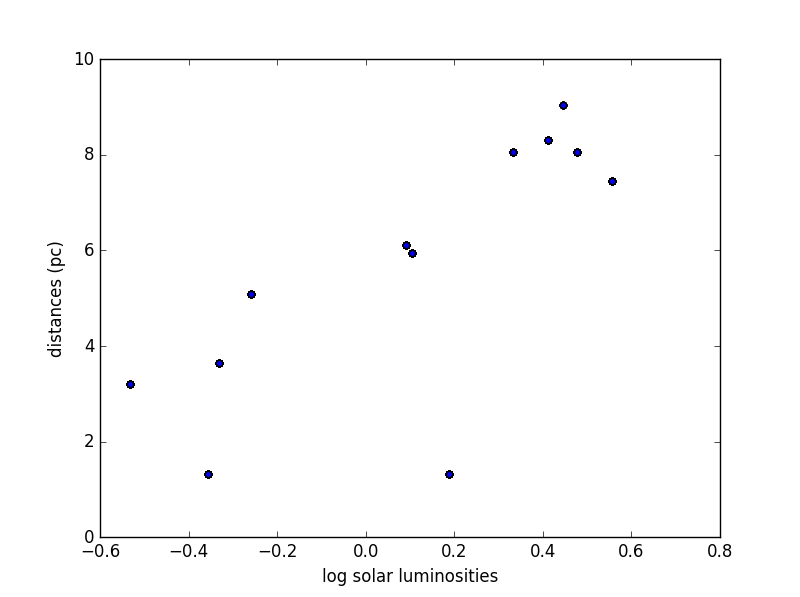
\includegraphics[width = \linewidth]{WFIRST_d_L_scatter.png}
		\caption{A scatter plot of the stars around which habitable zone exoplanets were detected in these simulations with WFIRST.}
		\label{fig:WFIRST_dL}
	\end{figure}
	
	\begin{figure}
		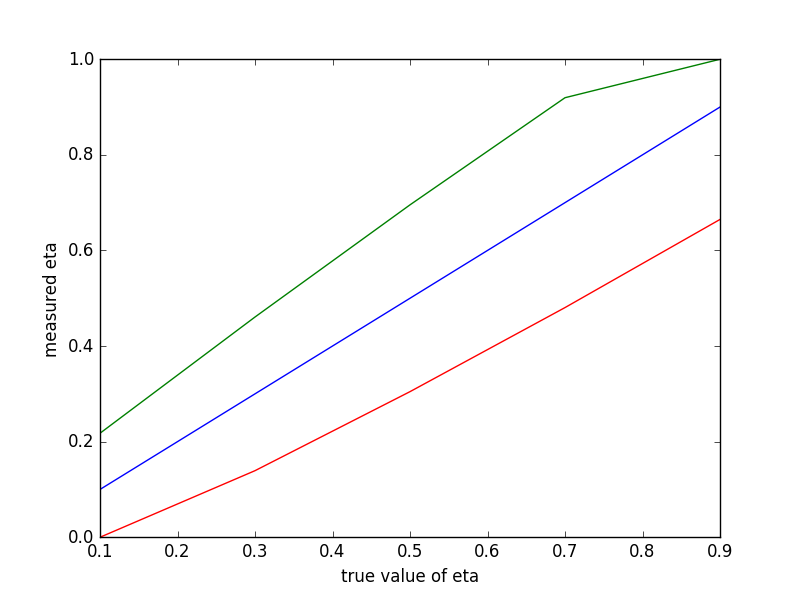
\includegraphics[width = \linewidth]{LUVOIR_eta_earth_constraints.png}
		\caption{95\% CI for $\eta_{Earth}$ as a function of the true value of $\eta_{Earth}$ for campaigns using LUVOIR.}
		\label{fig:LUVOIR_eta_constraints}
	\end{figure}
	
	\begin{figure}
		\includegraphics[width = \linewidth]{HABEX_eta_earth_constraints.png}
		\caption{95\% CI for $\eta_{Earth}$ as a function of the true value of $\eta_{Earth}$ for campaigns using HabEx.}
		\label{fig:HABEX_eta_constraints}
	\end{figure}
	
	
	We now run simulations looking at many prioritized stars assuming a campaign lifetime of one year. Each star is observed for $\tau_{ex}$ or until a planet is discovered. Planets are randomly generated around stars with a frequency $\eta_{Earth}$, a free parameter we vary in the simulations. We look at stars until the campaign lifetime has expired (1 year). For each value of $\eta_{Earth}$, we simulate many campaigns and collect statistics on the total number of habitable zone exoplanets found and the properties of the stars around which they were found (figures \ref{fig:LUVOIR_dL} and \ref{fig:WFIRST_dL}). 
	For each value of $\eta_{Earth}$, we also use a campaign simulation as a data set to create a confidence interval for the true value of $\eta_{Earth}$ (using the technique described in previous sections). We show the confidence interval provided in these simulations in figures \ref{fig:LUVOIR_eta_constraints} and \ref{fig:HABEX_eta_constraints}. We also record the number of planets found per $\eta_{Earth}$. The number of planets found is approximately linear with $\eta_{Earth}$. These assumed mission parameters are listed in figure \ref{fig:telescope}.
	
	\section{Appendix}
	\subsection{Comparison with Stark et al. 2014}
	
	\begin{figure}
		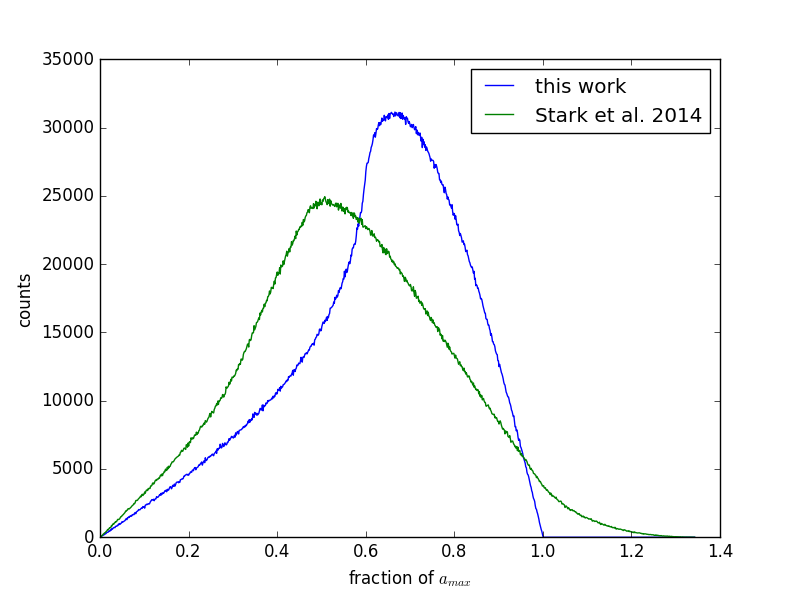
\includegraphics[width = \linewidth]{stark_compare.png}
		\caption{The results of an MC simulation that measures the apparent separation of habitable zone exoplanets are a fraction of the maximum semi-major axis.}
		\label{fig:stark_compare}
	\end{figure}
	
	Similar work has been done by Stark et al. 2014. They also observe with the intent of optimizing habitable zone exoplanet yield. They make different assumptions about the distribution of planets on the sky. The result of an MC simulation measuring apparent separation for both methods is shown in figure \ref{fig:stark_compare}. The main difference is that this work does not allow habitable zone orbits to ever exit the habitable zone and thus considers a smaller space of semi major axes and eccentricities. 
	
	\subsection{General code heuristics}

	Given below are some rules loosely adhered to in my code to help with reading it.
	
	\begin{itemize}
		\item editable free parameters are listed at the top of the code as class constants
		\item main function is always at the very bottom. In general functions are listed in order of their maximum position on the stack; i.e. functions that are put highest on the stack are at the top of the code
		\item typically variables normally named are matrices and variables followed by an underscore are specific values in a matrix; e.g. ``x`` would refer to the entire matrix, whereas ``x\_`` would refer to a specific value in that matrix; this convention is not the case for class attributes
		\item class attributes followed by an underscore typically refer to the same idea as another attribute but in a different circumstance; e.g. ``planet.x`` may be the x coordinate in 3 space and ``planet.x\_`` the x coordinate in the plane of the orbit 
		\item the naming convention in most of my code is to use underscoring as opposed to camelCasing
		\item ``Math`` is a homemade class that contains some functions that manipulate matrices but is mostly used to store the values of physical constants
	\end{itemize}
	
	\subsection{What code generates which figure?'}
	
	Figures \ref{e vs a} and \ref{a vs r} are made by ``plot\_bounds.py``. This program outputs three figures, the first is the region of integration in the $a$-$r$ plane. The second is the region of integration in the $a$-$e$ plane. The third is the aperture after a shear (it loads data from the given fits file).
	
	Figure \ref{fig:p_s} is made by ``pdf\_s.py``. Performs a Riemann sum to find the probability distribution for apparent separation. ``res`` is the only real important parameter to edit as it determines the resolution of the sum. I recommend keeping the resolution below 100, first of all because the program has runtime that is $O(res^4)$, and secondly because having an overly fine resolution will get the sum too close to divergences in the terms which do not properly converge when evaluating the sum discretely as we must do in a program. 
	
	Figures \ref{fig:MC} and \ref{fig:stark_compare} are made by ``s\_MC.py``. If ``stark`` is false then it outputs three figures. The first is a histogram of the separations. The second is the counts from each bin and a fit to them. The third has just the fit. If stark is true then a fourth figure compares the distribution from this work to the distribution from Stark's work. This will ruin the fit though so do not try and get figures comparing work and figures showing a reasonable fit at the same time. The last line of the code is commented out and outputs a pickle file containing the fit. 
	
	Figures \ref{fig:p_T}, \ref{T v wl}, and \ref{fig:T_xy2} are made by ``p\_T.py``. This program outputs three figures. The first is a histogram of the transmission for randomly generated positions on the sky choosing according to our probability distribution for on-sky separation. The second and third and transmission maps showing the transmission pattern created by various shears. 
	
	Figures \ref{fig:T v wl} and \ref{fig:z v wl} are made by ``P\_T\_all.pg``. This program outputs two figures. The first figure shows the average transmission as a function of wavelength. The second shows the probability of zero transmission as a function of wavelength.
	
	Figure \ref{fig:telescope} has information from a large number of sources. However the ``planets founds`` number comes from`` main3.py``. Figures \ref{fig:LUVOIR_dL}, \ref{fig:WFIRST_dL}, \ref{fig:LUVOIR_eta_constraints}, and \ref{fig:HABEX_eta_constraints} are also made using this program. The code runs a simulation of an observation campaign. It outputs eleven figures. The first, second, eight, and ninth are histograms of created and detected planets by the luminosity of their host stars, distance, semi major axis, and period, respectively. The third, fourth, tenth and eleventh are the fraction of created stars discovered as a function of luminosity, distance, semi major axis, and period, respectively. The fifth shows the z scores of discovered planets. Sixth shows a scatter plot of stars around which planets were found showing luminosity and distance. The seventh shows constrains put on eta as a function of the true value of eta.
	
	Figures \ref{fig:A_x} and \ref{fig:P_x_LUVOIR} are made by ``makePlots.py``. This program looks at the ability of a specific telescope to view stars within 30 pc. The program outputs two figures. The first shows how the IWA and OWA compare to the pdf for separation as a function of the observation parameter x. The second figure shows the probability of a random planet being inside the field of view as a function of the observation parameter and the number of stars with that observation parameter. 
	
	Figure \ref{fig:telescopes} is made by ``makePlots2.py``. This program outputs a figure showing a histogram of stars by their intrinsic observation parameter and the probability of a random habitable zone planet being inside the field of view as a function of the intrinsic observation parameter for a number of telescopes. 
	
	Figures \ref{fig:PI_} and \ref{fig:width} are made using ``MC\_eta.py``. This program uses the results of ``makePlots.py`` to calculate our ability to constrain the value of $\eta_{Earth}$ assuming that we visited each star within 30 pc and observed for $\tau_{ex}$. This program outputs two figures. The first shows a CI interval for $\eta$ by telescope, the second shows the width of that confidence interval both as a function of the true value of $\eta$. 
	
	Figures \ref{fig:LUVOIR_tau_ex}, \ref{fig:HABEX_tau_ex}, \ref{fig:WFIRST_tau_ex}, and \ref{fig:JWST_tau_ex} are made using ``find\_exclude.py``. The program outputs three figures. The last line is commented out and would output a pickle file containing the array of star objects representing the stars within 30 pc. Also prints out the top targets for this mission. The first and second output figures is a histogram of targets based on their $\tau_{ex}$ and proportion of detectable planets respectively. The third is a scatter plot comparing the two variables for each star.
	
	
\end{document}